%-------------------------------------------------------------------------------
\chapter[Cohesive sediment]{Cohesive sediment transport}
%-------------------------------------------------------------------------------

%-------------------------------------------------------------------------------
\section{Preliminaries}
%-------------------------------------------------------------------------------
Cohesive properties appear for fine particles (silts and clay), with diameter less than a limiting value of about 60 $\mu$m, depending on the physico-chemical 
properties of the fluid and salinity. The separation value at $60\mu$m to discriminate non-cohesive from cohesive sediment is conventional. This value is different depending on the country (e.g. $63\mu$m in The Netherlands, $75\mu$m in USA as pointed by Winterwerp and Van Kesteren~\cite{Winterwerp}). Moreover, aggregation of flocs can lead to the formation of macro-flocs larger than $100\mu$m.\\

Fine cohesive sediments are mainly transported in suspension and transport processes strongly depend on the state of floculation of the suspension and consolidation of the bed. The erosion rate mainly depends on the degree of consolidation of the sediment bed, while the settling velocity depends on the state of floculation and aggregates properties.\\

In \sisyphe{}, cohesive sediments are accounted by solving the 2D advection-diffusion equation:
\begin{equation*}
\frac{\partial hC}{\partial t} + \frac{\partial hUC}{\partial x} + \frac{\partial hVC}{\partial y} =
\frac{\partial}{\partial x}\left(h\epsilon_s\frac{\partial C}{\partial x}\right) +
\frac{\partial}{\partial y}\left(h\epsilon_s\frac{\partial C}{\partial y}\right) + (E-D)
\end{equation*}
$C=C(x,y,t)$ is the depth-averaged concentration \textcolor{black}{expressed in \% volume (-)}, $(U,V)$ are the depth-averaged components of the velocity in the $x$ and $y$ directions, respectively, $\epsilon_s$ is the turbulent diffusivity of the sediment.

The erosion flux is computed with the Partheniades formula:
\begin{equation*}
E = \left\{\begin{array}{ll}
M\left[\left(\frac{\tau_b}{\tau_{ce}}\right)-1\right]\quad & \text{if}\,\,\tau_b> \tau_{ce}\\  
0\quad & \text{otherwise}
\end{array}
\right. 
\end{equation*}
with $M$ the Krone-Partheniades erosion law constant [kg/m$^2$/s] and $\tau_{ce}$ the critical bed shear stress.

The deposition flux for mud is computed by the expression:
\begin{equation}
D = w_{s} C \left[1-\left(\frac{\sqrt{\tau_b/\rho}}{u_{*mud}^{cr}}\right)^2 \right],
\end{equation}
where $u_{*mud}^{cr}$ is the critical shear velocity for mud deposition.\\

The bed evolution is computed by:
\begin{equation*}
(1-\lambda)\frac{\partial z_b}{\partial t} = D - E
\end{equation*}
with $\lambda$ the bed porosity and $z_b$ bed level.

%-------------------------------------------------------------------------------
\section{Steering file setup for cohesive sediment transport}
%-------------------------------------------------------------------------------
In \sisyphe{}, the simplest case of cohesive sediments
is characterized by a uniform grain size $D_{50}\leq 60\,\mu$m which is
transported in suspension.

Cohesive sediments can be activated with the keyword {\ttfamily COHESIVE SEDIMENTS = YES} (logical type, set to {\ttfamily = NO} by default). When {\ttfamily COHESIVE SEDIMENTS = YES}, the following keywords are set automatically to keep consistency with the selected type of sediment: {\ttfamily SUSPENSION = YES} and {\ttfamily BED LOAD = NO}.


%-------------------------------------------------------------------------------
\section{Initialization of the bed structure}
%-------------------------------------------------------------------------------
The cohesive sediment bed can be represented by a fixed number of layers ($<20$) with the keyword {\ttfamily NUMBER OF LAYERS OF THE CONSOLIDATION MODEL} (integer type, set to {\ttfamily = 1} by default).

Each layer is characterized by its concentration and resistance to the erosion. The concentration of each layer $C_s$ is generally constant and can be specified with the keyword {\ttfamily MUD CONCENTRATION PER LAYER} (real list, set to {\ttfamily = 50.;100.;150.;...} by default), expressed in kg/m$^3$ or gr/l.

The resistance of each layer can be specified with the keyword {\ttfamily CRITICAL EROSION SHEAR STRESS OF THE MUD} (real list, set to {\ttfamily = 0.01;0.02;0.03;...} by default), expressed in N/m$^2$.

The initialization can also be done with the subroutine \texttt{init\_compo\_coh.f}.

\begin{figure}[H]%
\begin{center}
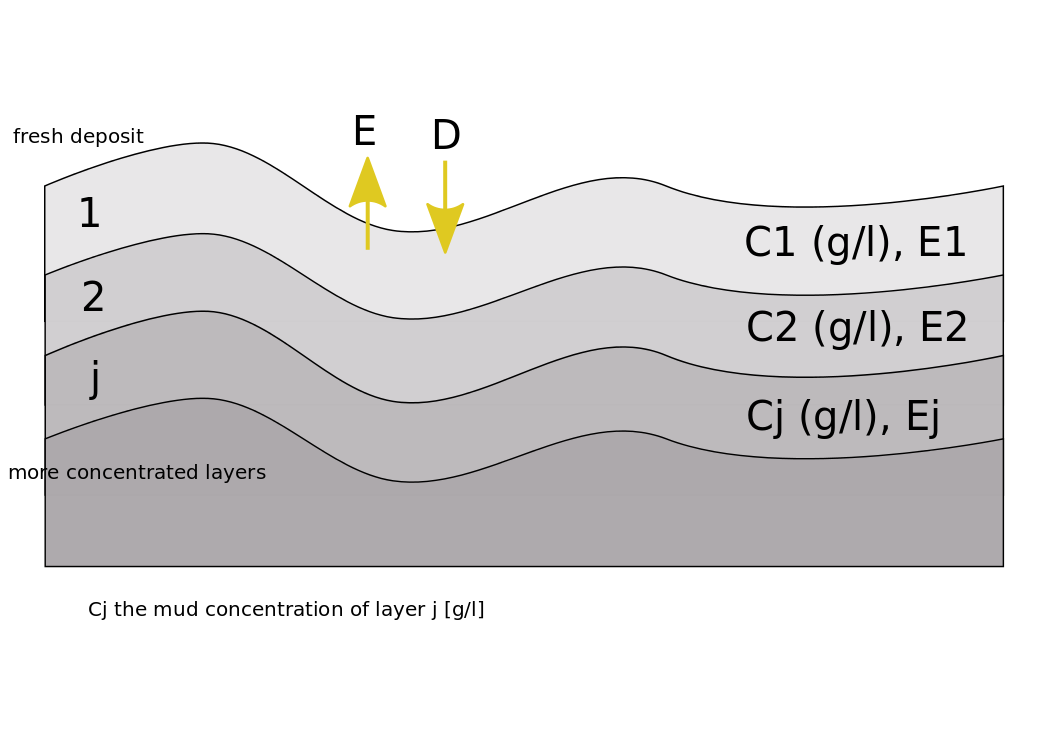
\includegraphics[scale=0.3]{./graphics/consolidation.png}
\end{center}
\end{figure}

%-------------------------------------------------------------------------------
\section{Properties of the cohesive sediments}
%-------------------------------------------------------------------------------
The keywords {\ttfamily NUMBER OF BED LOAD MODEL LAYERS} (for non-cohesive sediments) and {\ttfamily NUMBER OF LAYERS OF THE CONSOLIDATION MODEL} are essentially the same except that the default values are different.

For cohesive sediments, it is possible to have only one uniform layer, whereas for non-cohesive sand grading we need at least two layers (the active layer and the stratum).


%-------------------------------------------------------------------------------
\subsection{Erosion flux}
%-------------------------------------------------------------------------------
The erosion flux is computed with the Partheniades formula. For uniform beds, the erosion flux is related to the excess of
applied bed shear stress to the bed shear strength at the bed surface:
\begin{equation*}
E = \left\{\begin{array}{ll}
M\left[\left(\frac{\tau_b}{\tau_{ce}}\right)-1\right]\quad & \text{if}\,\,\tau_b> \tau_{ce}\\  
0\quad & \text{otherwise}
\end{array}
\right. 
\end{equation*}
where $M$ the Krone-Partheniades erosion law constant [kg/m$^2$/s] is provided by the keyword {\ttfamily PARTHENIADES CONSTANT} (real type, set to {\ttfamily = 1.E-03} by default).

The value of $\tau_{ce}$ can be provided for the different layers with the keyword {\ttfamily CRITICAL EROSION SHEAR STRESS OF THE MUD} (real list, set to {\ttfamily = 0.01;0.02;0.03;...} by default), expressed in N/m$^2$.

%-------------------------------------------------------------------------------
\subsection{Deposition flux}
%-------------------------------------------------------------------------------
The deposition flux for mud is computed by the expression:
\begin{equation}
D = w_{s} C \left[1-\left(\frac{\sqrt{\tau_b/\rho}}{u_{*mud}^{cr}}\right)^2 \right],
\end{equation}
where $u_{*mud}^{cr}$ is the critical shear velocity for mud deposition, expressed in [m/s] and provided by the keyword {\ttfamily CRITICAL SHEAR VELOCITY FOR MUD DEPOSITION} (real type, set to {\ttfamily = 1000.} by default).

For the evaluation of the settling velocity $w_s $, if the keyword {\ttfamily SETTLING VELOCITIES} is not included in the steering file, \sisyphe{} computes the settling velocity for each sediment class by the Stokes, Zanke or van Rijn formulae depending on the grain size. For further details see the subroutine \texttt{vitchu\_sisyphe.f}.

%-------------------------------------------------------------------------------
\section{Consolidation processes}
%-------------------------------------------------------------------------------
The keyword {\ttfamily MUD CONSOLIDATION} (logical type, set to {\ttfamily = NO} by default) activates consolidation processes in \sisyphe{}. Two different models for consolidation are available with the keyword {\ttfamily CONSOLIDATION MODEL} (logical type, set to {\ttfamily = 1} by default):
\begin{itemize}
\item Multilayer model ({\ttfamily = 1}): This empirical model assumes that the vertical flux of
sediment from layer $j$ to underneath layer $j+1$ is proportional to the mass of
sediments $M_s$ contained in the layer $j$.
\item The Gibson/Thiebot's model ({\ttfamily = 2}): the sediment flux from one layer
to another is computed from the Gibson theory.
\end{itemize}

Further information about both models can be found in~\cite{Lan12}.

\subsection{Associated keywords for consolidation models}
\begin{itemize}
\item Multilayer model ({\ttfamily = 1})
\begin{itemize}
\item {\ttfamily MASS TRANSFER PER LAYER} (real list, set to {\ttfamily = 5.D-05;4.5D-05;...} by default) provides the mass transfert coefficients of the multilayer consolidation model %UNITSSSS??????
\end{itemize} 
\item The Gibson/Thiebot's model ({\ttfamily = 2})
\begin{itemize}
\item {\ttfamily GEL CONCENTRATION} (real type, set to {\ttfamily = 310.D0} kg/m$^3$ by default)
\item {\ttfamily MAXIMUM CONCENTRATION} (real type, set to {\ttfamily = 364.D0} kg/m$^3$ by default)
\item {\ttfamily PERMEABILITY COEFFICIENT} (real type, set to {\ttfamily = 8.D0} by default) %CHECK IF OK FOR MODEL 2 AND UNITS?
\end{itemize}
\end{itemize} 

%-------------------------------------------------------------------------------
\section{Useful graphical printouts}
%-------------------------------------------------------------------------------
Some useful printouts for cohesive sediments are available by activating {\ttfamily VARIABLES FOR GRAPHIC PRINTOUTS}:
\begin{lstlisting}[frame=trBL]  
kES="thickness of the k layer";
kCONC="concentration of bed layer k";
CSi="concentration volumic or mass concentration 
for class i";
\end{lstlisting}  
Examples of use: \texttt{*ES,**ES,*CONC,**CONC,CS1}.
